\chapter{\Penrose{} Registry Benchmark}
\label{app:registry-benchmark}

As described in \cref{sec:penrose-open-source}, the \Penrose{} repository includes continuous integration tests that compile, render, and benchmark a large set of diagrams for every commit to the repository. This is a sample from commit \texttt{d3c6dd0ab42d4f6fe64fa47f2ac5a1660c8e552e} in the \texttt{penrose/penrose} GitHub repository.

\section{Data}
\begin{longtable}{|p{6.5cm}|c|c|c|c|}
    \hline
    \textbf{Diagram ID} & \textbf{Compile (s)} & \textbf{Optimize (s)} & \textbf{Render (s)} & \textbf{Total (s)} \endhead \hline
    \texttt{set-theory-domain/tree-euler} & 0.1617 & 0.0623 & 0.0307 & 0.2860 \\ \hline
    \texttt{set-theory-domain/tree-tree} & 0.1040 & 0.0441 & 0.0219 & 0.1790 \\ \hline
    \texttt{group-theory/quaternion-multiplication-table} & 0.4016 & 0.0079 & 0.1948 & 0.6215 \\ \hline
    \texttt{walk-on-spheres/SignedAngleOutside} & 0.3892 & 0.0076 & 0.0330 & 0.4783 \\ \hline
    \texttt{spectral-graphs/examples/hypercube} & 0.2600 & 0.0629 & 0.0244 & 0.3596 \\ \hline
    \texttt{group-theory/quaternion-cayley-graph} & 0.1219 & 0.0144 & 0.0200 & 0.1633 \\ \hline
    \texttt{set-theory-domain/tree-euler-3d} & 0.0849 & 0.0624 & 0.0735 & 0.2279 \\ \hline
    \texttt{atoms-and-bonds/one-water-molecule} & 0.0381 & 0.0035 & 0.0060 & 0.0577 \\ \hline
    \texttt{structural-formula/molecules/caffeine} & 0.4092 & 0.2345 & 0.1633 & 0.8212 \\ \hline
    \texttt{walk-on-spheres/walk-on-stars} & 0.6441 & 0.1326 & 0.4755 & 1.2861 \\ \hline
    \texttt{set-theory-domain/continuousmap} & 0.0702 & 0.0116 & 0.0106 & 0.1047 \\ \hline
    \texttt{mobius/mobius} & 0.0728 & 0.0451 & 0.0290 & 0.1587 \\ \hline
    \texttt{linear-algebra-domain/two-vectors-perp} & 0.0597 & 0.0054 & 0.0059 & 0.0853 \\ \hline
    \texttt{tutorials/tutorial1} & 0.0080 & 0.0003 & 0.0011 & 0.0215 \\ \hline
    \texttt{tutorials/tutorial2} & 0.0055 & 0.0001 & 0.0005 & 0.0163 \\ \hline
    \texttt{tutorials/tutorial3} & 0.0214 & 0.0003 & 0.0031 & 0.0341 \\ \hline
    \texttt{molecules/nitricacid-lewis} & 0.2605 & 0.0810 & 0.0115 & 0.3746 \\ \hline
    \texttt{array-models/insertionSort} & 0.3978 & 0.0180 & 0.1119 & 0.5422 \\ \hline
    \texttt{exterior-algebra/vector-wedge} & 0.0566 & 0.0051 & 0.0066 & 0.0791 \\ \hline
    \texttt{shape-spec/all-shapes} & 0.0736 & 0.0009 & 0.4533 & 0.5397 \\ \hline
    \texttt{shape-spec/arrowheads} & 0.0407 & 0.0021 & 0.0128 & 0.0643 \\ \hline
    \texttt{graph-domain/textbook/sec1/fig1} & 0.2401 & 0.2027 & 0.0120 & 0.4653 \\ \hline
    \texttt{graph-domain/textbook/sec1/fig2} & 0.2789 & 0.3640 & 0.0084 & 0.6626 \\ \hline
    \texttt{graph-domain/textbook/sec1/fig3} & 0.2997 & 0.4485 & 0.0104 & 0.7645 \\ \hline
    \texttt{graph-domain/textbook/sec1/fig4} & 0.3430 & 0.4748 & 0.0175 & 0.8461 \\ \hline
    \texttt{spectral-graphs/examples/hexagonal-lattice} & 2.5054 & 0.4903 & 0.1132 & 3.1165 \\ \hline
    \texttt{dinoshade/dinoshade} & 1.0746 & 0.0009 & 0.1289 & 1.2471 \\ \hline
    \texttt{spectral-graphs/examples/star-graph} & 2.9737 & 0.0925 & 0.0651 & 3.1643 \\ \hline
    \texttt{spectral-graphs/examples/box} & 1.9651 & 0.0894 & 0.0737 & 2.1570 \\ \hline
    \texttt{graph-domain/textbook/sec1/fig5} & 0.3582 & 0.6457 & 0.0132 & 1.0435 \\ \hline
    \texttt{graph-domain/textbook/sec1/fig6} & 1.1834 & 2.6696 & 0.0156 & 3.8756 \\ \hline
    \texttt{graph-domain/textbook/sec1/fig7} & 0.1558 & 0.1536 & 0.0080 & 0.3232 \\ \hline
    \texttt{graph-domain/textbook/sec1/fig8a} & 0.4356 & 0.6583 & 0.0130 & 1.1136 \\ \hline
    \texttt{graph-domain/textbook/sec1/fig8b} & 0.2841 & 0.5315 & 0.0092 & 0.8318 \\ \hline
    \texttt{graph-domain/textbook/sec1/fig9} & 0.2205 & 0.2046 & 0.0192 & 0.4504 \\ \hline
    \texttt{graph-domain/textbook/sec1/fig10} & 0.2041 & 0.0820 & 0.0868 & 0.3805 \\ \hline
    \texttt{graph-domain/textbook/sec1/fig11} & 0.2947 & 0.1851 & 0.1356 & 0.6218 \\ \hline
    \texttt{graph-domain/textbook/sec1/fig12} & 0.3658 & 0.3410 & 0.1034 & 0.8170 \\ \hline
    \texttt{graph-domain/textbook/sec1/fig13} & 0.3410 & 0.4390 & 0.0116 & 0.7982 \\ \hline
    \texttt{graph-domain/textbook/sec2/fig3} & 0.5993 & 1.7477 & 0.0198 & 2.3737 \\ \hline
    \texttt{graph-domain/textbook/sec2/fig4} & 0.4177 & 0.9079 & 0.0158 & 1.3481 \\ \hline
    \texttt{graph-domain/textbook/sec2/fig5} & 0.6763 & 1.6441 & 0.0223 & 2.3497 \\ \hline
    \texttt{graph-domain/textbook/sec2/fig6} & 0.5970 & 1.2551 & 0.0129 & 1.8715 \\ \hline
    \texttt{graph-domain/textbook/sec2/fig9} & 1.0244 & 2.7261 & 0.0341 & 3.7915 \\ \hline
    \texttt{graph-domain/textbook/sec2/fig10a} & 0.2164 & 0.3068 & 0.0071 & 0.5362 \\ \hline
    \texttt{graph-domain/textbook/sec2/fig10b} & 0.2008 & 0.1741 & 0.0600 & 0.4415 \\ \hline
    \texttt{graph-domain/textbook/sec2/fig11a} & 0.1391 & 0.0262 & 0.0445 & 0.2173 \\ \hline
    \texttt{graph-domain/textbook/sec2/fig11b} & 0.1152 & 0.0194 & 0.0323 & 0.1729 \\ \hline
    \texttt{graph-domain/textbook/sec2/fig11c} & 0.1417 & 0.0551 & 0.0676 & 0.2703 \\ \hline
    \texttt{graph-domain/textbook/sec2/fig12} & 0.1248 & 0.0274 & 0.0526 & 0.2116 \\ \hline
    \texttt{graph-domain/textbook/sec2/fig13} & 1.0088 & 2.2440 & 0.0145 & 3.2750 \\ \hline
    \texttt{graph-domain/textbook/sec2/fig14} & 0.2433 & 0.2700 & 0.0242 & 0.5450 \\ \hline
    \texttt{graph-domain/textbook/sec2/fig16b} & 0.1621 & 0.0281 & 0.0543 & 0.2519 \\ \hline
    \texttt{geometry-domain/textbook\_problems/c05p13} & 0.2135 & 0.0769 & 0.0070 & 0.3308 \\ \hline
    \texttt{geometry-domain/textbook\_problems/c01p01} & 0.2054 & 0.0761 & 0.0064 & 0.2944 \\ \hline
    \texttt{geometry-domain/textbook\_problems/c03p01} & 0.2099 & 0.0671 & 0.0078 & 0.2906 \\ \hline
    \texttt{geometry-domain/textbook\_problems/c05p01} & 0.2103 & 0.0503 & 0.0079 & 0.2740 \\ \hline
    \texttt{geometry-domain/textbook\_problems/ex} & 0.2727 & 0.1528 & 0.0190 & 0.4504 \\ \hline
    \texttt{triangle-mesh-3d/two-triangles} & 0.1617 & 0.0239 & 0.0524 & 0.2540 \\ \hline
    \texttt{random-sampling/test} & 0.3614 & 0.0257 & 0.0268 & 0.4265 \\ \hline
    \texttt{geometry-domain/textbook\_problems/c11p12} & 0.2405 & 0.1207 & 0.0085 & 0.3785 \\ \hline
    \texttt{molecules/sulfuric-acid} & 0.2970 & 0.1172 & 0.0082 & 0.4290 \\ \hline
    \texttt{curve-examples/catmull-rom/catmull-rom} & 0.0492 & 0.0387 & 0.0075 & 0.1099 \\ \hline
    \texttt{word-cloud/example} & 0.1680 & 0.2567 & 0.0121 & 0.4469 \\ \hline
    \texttt{geometry-domain/siggraph-teaser} & 0.2532 & 0.0870 & 0.0224 & 0.3838 \\ \hline
    \texttt{minkowski-tests/maze/non-convex} & 0.0883 & 0.0753 & 0.0019 & 0.1759 \\ \hline
    \texttt{lagrange-bases/lagrange-bases} & 0.0735 & 0.0371 & 0.0679 & 0.1929 \\ \hline
    \texttt{hypergraph/hypergraph} & 0.3398 & 1.8090 & 0.0260 & 2.1863 \\ \hline
    \texttt{persistent-homology/persistent-homology} & 0.2384 & 0.9388 & 0.1117 & 1.3130 \\ \hline
    \texttt{walk-on-spheres/laplace-estimator} & 0.2168 & 0.0508 & 0.0575 & 0.3315 \\ \hline
    \texttt{walk-on-spheres/poisson-estimator} & 0.2304 & 0.0563 & 0.0452 & 0.3378 \\ \hline
    \texttt{walk-on-spheres/nested-estimator} & 0.3070 & 0.0901 & 0.0929 & 0.4969 \\ \hline
    \texttt{walk-on-spheres/offcenter-estimator} & 0.2174 & 0.0393 & 0.0546 & 0.3172 \\ \hline
    \texttt{shape-distance/points-around-star} & 0.2239 & 0.0160 & 0.0127 & 0.2649 \\ \hline
    \texttt{shape-distance/points-around-polyline} & 0.1556 & 0.0195 & 0.0125 & 0.1947 \\ \hline
    \texttt{shape-distance/points-around-line} & 0.1349 & 0.0083 & 0.0133 & 0.1626 \\ \hline
    \texttt{shape-distance/lines-around-rect} & 0.0585 & 0.0146 & 0.0193 & 0.1002 \\ \hline
    \texttt{fake-3d-linear-algebra/projection} & 0.0442 & 0.0091 & 0.0031 & 0.0670 \\ \hline
    \texttt{animation/center-shrink-circle} & 0.0149 & 0.0095 & 0.0070 & 0.0425 \\ \hline
    \texttt{graph-domain/other-examples/hamiltonian-cycle} & 0.2869 & 0.4041 & 0.0106 & 0.7075 \\ \hline
    \texttt{structural-formula/reactions/methane-combustion} & 0.3364 & 1.0808 & 0.0373 & 1.4689 \\ \hline
    \texttt{molecules/glutamine} & 0.1487 & 0.0494 & 0.0713 & 0.2785 \\ \hline
    \texttt{matrix-ops/tests/matrix-matrix-addition} & 0.0923 & 0.0010 & 0.0121 & 0.1231 \\ \hline
    \texttt{matrix-ops/tests/matrix-matrix-division-elementwise} & 0.0927 & 0.0010 & 0.0106 & 0.1103 \\ \hline
    \texttt{matrix-ops/tests/matrix-matrix-multiplication-elementwise} & 0.0910 & 0.0010 & 0.0117 & 0.1093 \\ \hline
    \texttt{matrix-ops/tests/matrix-matrix-multiplication} & 0.0912 & 0.0010 & 0.0102 & 0.1084 \\ \hline
    \texttt{matrix-ops/tests/matrix-matrix-subtraction} & 0.0984 & 0.0017 & 0.0151 & 0.1206 \\ \hline
    \texttt{matrix-ops/tests/matrix-transpose} & 0.0850 & 0.0009 & 0.0074 & 0.0992 \\ \hline
    \texttt{matrix-ops/tests/matrix-vector-left-multiplication} & 0.0822 & 0.0008 & 0.0074 & 0.0960 \\ \hline
    \texttt{matrix-ops/tests/matrix-vector-right-multiplication} & 0.0834 & 0.0009 & 0.0071 & 0.0968 \\ \hline
    \texttt{matrix-ops/tests/scalar-vector-division} & 0.0864 & 0.0008 & 0.0106 & 0.1037 \\ \hline
    \texttt{matrix-ops/tests/scalar-vector-left-multiplication} & 0.0812 & 0.0008 & 0.0079 & 0.0961 \\ \hline
    \texttt{matrix-ops/tests/scalar-vector-right-multiplication} & 0.0810 & 0.0012 & 0.0072 & 0.0959 \\ \hline
    \texttt{matrix-ops/tests/vector-vector-addition} & 0.0851 & 0.0015 & 0.0111 & 0.1036 \\ \hline
    \texttt{matrix-ops/tests/vector-vector-division-elementwise} & 0.0904 & 0.0012 & 0.0077 & 0.1053 \\ \hline
    \texttt{matrix-ops/tests/vector-vector-multiplication-elementwise} & 0.0833 & 0.0008 & 0.0080 & 0.0976 \\ \hline
    \texttt{matrix-ops/tests/vector-vector-outerproduct} & 0.0950 & 0.0009 & 0.0093 & 0.1109 \\ \hline
    \texttt{matrix-ops/tests/vector-vector-subtraction} & 0.0860 & 0.0009 & 0.0060 & 0.0982 \\ \hline
    \texttt{logic-circuit-domain/half-adder} & 0.1062 & 0.0655 & 0.0108 & 0.1967 \\ \hline
    \texttt{curve-examples/cubic-bezier} & 0.0923 & 0.3887 & 0.0101 & 0.5018 \\ \hline
    \texttt{triangle-mesh-2d/diagrams/cotan-formula} & 0.1652 & 0.0991 & 0.0100 & 0.2949 \\ \hline
    \texttt{triangle-mesh-2d/diagrams/concyclic-pair} & 0.1682 & 0.1122 & 0.0109 & 0.2969 \\ \hline
    \texttt{triangle-mesh-2d/diagrams/halfedge-mesh} & 0.1538 & 0.0165 & 0.0190 & 0.1955 \\ \hline
    \texttt{triangle-mesh-2d/diagrams/relative-orientation} & 0.1464 & 0.0257 & 0.0089 & 0.1873 \\ \hline
    \texttt{triangle-mesh-2d/diagrams/triangle-centers} & 0.1400 & 0.0186 & 0.0058 & 0.1709 \\ \hline
    \texttt{triangle-mesh-2d/diagrams/angle-equivalence} & 0.2231 & 0.3366 & 0.0189 & 0.5857 \\ \hline
    \texttt{timeline/penrose} & 0.3208 & 0.0925 & 0.1516 & 0.5773 \\ \hline
    \texttt{graph-domain/textbook/sec5/ex32} & 0.7038 & 3.1439 & 0.0475 & 3.9046 \\ \hline
    \texttt{curve-examples/open-elastic-curve} & 0.1996 & 0.2155 & 0.0052 & 0.4279 \\ \hline
    \texttt{curve-examples/closed-elastic-curve} & 0.1978 & 0.2665 & 0.0037 & 0.4753 \\ \hline
    \texttt{graph-domain/other-examples/arpanet} & 0.6853 & 2.8871 & 0.0568 & 3.6410 \\ \hline
    \texttt{graph-domain/other-examples/nyc-subway} & 0.8933 & 2.1443 & 0.0386 & 3.0854 \\ \hline
    \texttt{fancy-text/fancy-text} & 0.1992 & 0.2492 & 0.0196 & 0.4784 \\ \hline
    \texttt{curve-examples/blobs} & 0.7099 & 4.3173 & 0.0218 & 5.0689 \\ \hline
    \texttt{curve-examples/space-curves} & 0.6714 & 0.5937 & 0.0158 & 1.3451 \\ \hline
    \texttt{geometric-queries/ray-intersect/test-group} & 0.6447 & 0.0112 & 0.0477 & 0.7143 \\ \hline
    \texttt{ray-tracing/path-trace} & 0.0853 & 0.0008 & 0.0203 & 0.1231 \\ \hline
    \texttt{ray-tracing/bidirectional} & 0.1011 & 0.0010 & 0.0156 & 0.1238 \\ \hline
    \texttt{ray-tracing/next-event-estimation} & 0.1126 & 0.0125 & 0.0723 & 0.2038 \\ \hline
    \texttt{geometric-queries/test} & 0.2136 & 0.0125 & 0.0217 & 0.2630 \\ \hline
    \texttt{geometric-queries/closest-point/test-group} & 0.1064 & 0.0299 & 0.0164 & 0.1650 \\ \hline
    \texttt{geometric-queries/closest-point/test} & 0.0606 & 0.0028 & 0.0041 & 0.0737 \\ \hline
    \texttt{geometric-queries/closest-silhouette-point/test} & 0.0639 & 0.0015 & 0.0062 & 0.0842 \\ \hline
    \texttt{geometric-queries/ray-intersect/test} & 0.5821 & 0.0230 & 0.0552 & 0.6706 \\ \hline
    \texttt{box-arrow-diagram/computer-architecture} & 0.7727 & 3.5983 & 0.0328 & 4.4158 \\ \hline
    \texttt{stochastic-process/stochastic-process} & 2.9791 & 0.0211 & 0.3926 & 3.4046 \\ \hline
    \texttt{stochastic-process/epsilon-shell/AbsorbingBoundary} & 1.7551 & 0.0199 & 0.1634 & 1.9586 \\ \hline
    \texttt{solid/eigenspace} & - & - & - & 0.1424 \\ \hline
    \texttt{solid/triangles} & - & - & - & 0.0621 \\ \hline
    \texttt{solid/vectors} & - & - & - & 0.0559 \\ \hline
    \texttt{tsne/tsne} & 1.0705 & 1.6735 & 0.0540 & 2.8082 \\ \hline
    \texttt{spectral-graphs/examples/4x4-sudoku-graph} & 0.2802 & 0.0782 & 0.0423 & 0.4081 \\ \hline
    \texttt{spectral-graphs/examples/dodecahedral-graph} & 0.1783 & 0.0531 & 0.0223 & 0.2598 \\ \hline
    \texttt{matrix-library/crossProductMatrix} & 0.0463 & 0.0002 & 0.0047 & 0.0684 \\ \hline
    \texttt{matrix-library/diagonal2d} & 0.0255 & 0.0002 & 0.0018 & 0.0415 \\ \hline
    \texttt{matrix-library/diagonal3d} & 0.0484 & 0.0002 & 0.0033 & 0.0585 \\ \hline
    \texttt{matrix-library/identity2d} & 0.0259 & 0.0002 & 0.0017 & 0.0333 \\ \hline
    \texttt{matrix-library/identity3d} & 0.0781 & 0.0002 & 0.0050 & 0.0891 \\ \hline
    \texttt{matrix-library/inverse2d} & 0.0262 & 0.0002 & 0.0018 & 0.0344 \\ \hline
    \texttt{matrix-library/inverse3d} & 0.0477 & 0.0002 & 0.0041 & 0.0573 \\ \hline
    \texttt{matrix-library/matrix2d} & 0.0271 & 0.0002 & 0.0019 & 0.0349 \\ \hline
    \texttt{matrix-library/matrix3d} & 0.0460 & 0.0002 & 0.0048 & 0.0566 \\ \hline
    \texttt{matrix-library/outerProduct2d} & 0.0315 & 0.0002 & 0.0018 & 0.0408 \\ \hline
    \texttt{matrix-library/outerProduct3d} & 0.0476 & 0.0002 & 0.0032 & 0.0564 \\ \hline
    \texttt{matrix-library/rotate} & 0.0262 & 0.0002 & 0.0018 & 0.0335 \\ \hline
    \texttt{matrix-library/rotate2d} & 0.0261 & 0.0002 & 0.0018 & 0.0332 \\ \hline
    \texttt{matrix-library/rotate3d} & 0.0493 & 0.0002 & 0.0033 & 0.0583 \\ \hline
    \texttt{matrix-library/rotate3dh} & 0.0493 & 0.0002 & 0.0043 & 0.0591 \\ \hline
    \texttt{matrix-library/scale2d} & 0.0258 & 0.0002 & 0.0017 & 0.0337 \\ \hline
    \texttt{matrix-library/scale3d} & 0.0454 & 0.0002 & 0.0047 & 0.0557 \\ \hline
    \texttt{matrix-library/shear2d} & 0.0244 & 0.0002 & 0.0017 & 0.0313 \\ \hline
    \texttt{matrix-library/shear3d} & 0.0476 & 0.0002 & 0.0032 & 0.0566 \\ \hline
    \texttt{matrix-library/skew2d} & 0.0270 & 0.0002 & 0.0017 & 0.0346 \\ \hline
    \texttt{matrix-library/translate2d} & 0.0245 & 0.0002 & 0.0017 & 0.0318 \\ \hline
    \texttt{matrix-library/translate3dh} & 0.0481 & 0.0002 & 0.0030 & 0.0567 \\ \hline
    \texttt{atoms-and-bonds/wet-floor} & 0.0817 & 0.1964 & 0.0133 & 0.3020 \\ \hline
    \texttt{curve-examples/offset} & 0.0715 & 0.1809 & 0.0149 & 0.2761 \\ \hline
    \texttt{curve-examples/frenet-frame} & 0.0652 & 0.0665 & 0.0163 & 0.1572 \\ \hline
    \texttt{curve-examples/osculating-circle} & 0.0386 & 0.0386 & 0.0035 & 0.0883 \\ \hline
    \texttt{curve-examples/evolute-of-cardioid} & 0.4176 & 0.0018 & 0.0248 & 0.4511 \\ \hline
    \texttt{spectral-graphs/examples/truncated-cube-graph} & 0.2267 & 0.0348 & 0.0195 & 0.2906 \\ \hline
    \texttt{spectral-graphs/examples/torus} & 4.2913 & 0.2571 & 0.0978 & 4.6534 \\ \hline
    \texttt{spectral-graphs/examples/mobius} & 3.6053 & 0.3229 & 0.0775 & 4.0122 \\ \hline
    \texttt{impossible-ngon/ngon} & 1.0286 & 0.0024 & 0.1594 & 1.2033 \\ \hline
    \texttt{impossible-ngon/parameters} & 0.0456 & 0.0005 & 0.0061 & 0.0632 \\ \hline
    \texttt{impossible-ngon/nsides-chirality} & 0.2108 & 0.0027 & 0.0735 & 0.2989 \\ \hline
    \texttt{spectral-graphs/examples/periodic-hexagonal-lattice} & 1.1223 & 0.1776 & 0.0368 & 1.3448 \\ \hline
    \texttt{alloy-models/dining-philosophers} & 0.1903 & 0.0012 & 0.0088 & 0.2465 \\ \hline
    \texttt{alloy-models/message-passing} & 0.1825 & 0.6364 & 0.0241 & 0.8554 \\ \hline
    \texttt{alloy-models/ring-leader-election} & 0.0632 & 0.0531 & 0.0082 & 0.1370 \\ \hline
    \texttt{alloy-models/river-crossing} & 0.0316 & 0.0026 & 0.3057 & 0.3518 \\ \hline
    \texttt{alloy-models/workstations} & 0.1052 & 0.2446 & 0.0180 & 0.3799 \\ \hline
    \texttt{alloy-models/generic} & 0.4811 & 1.5036 & 0.0173 & 2.0151 \\ \hline
    \texttt{Dynamics/Lyapunov} & 0.0475 & 0.0036 & 0.0093 & 0.0716 \\ \hline
    \texttt{fractals/chaos-game/sierpinski-triangle} & 1.4528 & 0.1112 & 0.5393 & 2.1141 \\ \hline
    \texttt{fractals/chaos-game/vicsek-fractal} & 2.0627 & 0.2556 & 0.5438 & 2.8707 \\ \hline
    \texttt{fractals/l-systems/tree} & 0.3863 & 0.0021 & 0.0925 & 0.4907 \\ \hline
    \texttt{fractals/ifs/ifs} & 1.6085 & 0.0252 & 0.5028 & 2.1466 \\ \hline
    \texttt{envelopes/nephroid} & 0.3775 & 0.0676 & 0.0705 & 0.5256 \\ \hline
    \texttt{dataviz/linearreg} & 0.0484 & 0.0017 & 0.0075 & 0.0676 \\ \hline
    \texttt{dataviz/residual} & 0.0266 & 0.0017 & 0.0026 & 0.0397 \\ \hline
    \texttt{geometry-domain/complementary-angles} & 0.1802 & 0.2930 & 0.0084 & 0.4983 \\ \hline
    \texttt{alloy-models/icicle-plot-file-system} & 0.1116 & 0.0176 & 0.0216 & 0.1622 \\ \hline
    \texttt{interactive/ellipse-rays} & 0.5733 & 0.0033 & 0.0921 & 0.6794 \\ \hline
    \texttt{interactive/viewport} & 0.7039 & 0.2762 & 0.0156 & 1.0459 \\ \hline
    \texttt{interactive/planets} & 0.0189 & 0.0019 & 0.0081 & 0.0391 \\ \hline
    \texttt{set-potatoes/relation-not-a-function} & 0.0530 & 0.0055 & 0.0067 & 0.1161 \\ \hline
    \texttt{set-potatoes/injections-post-inverses} & 0.0932 & 0.0626 & 0.0135 & 0.1764 \\ \hline
    \texttt{set-potatoes/non-injection-not-monomorphism} & 0.1130 & 0.0909 & 0.0165 & 0.2279 \\ \hline
    \texttt{set-potatoes/surjections-pre-inverses} & 0.1328 & 0.0563 & 0.0152 & 0.2119 \\ \hline
    \texttt{set-potatoes/non-surjection-not-epimorphism} & 0.1104 & 0.2924 & 0.0253 & 0.4517 \\ \hline
\end{longtable}


\chapter{\Penrose{} Registry Diagrams}
\label{app:registry-diagram}

This section includes all diagrams rendered by commit \texttt{d3c6dd0ab42d4f6fe64fa47f2ac5a1660c8e552e} in \texttt{penrose/penrose}. Related performance data can be found in \cref{app:registry-benchmark}.

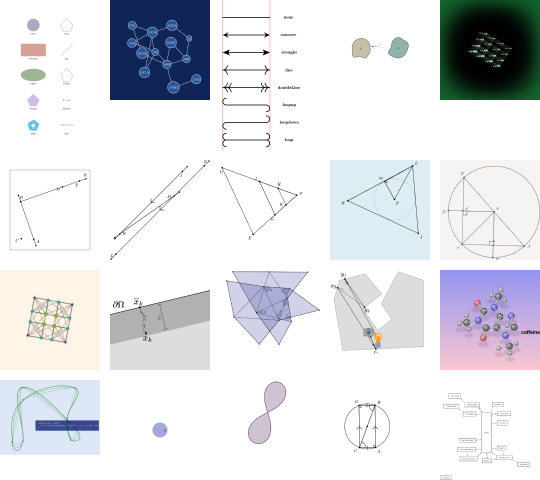
\includegraphics[width=\linewidth]{assets/appendix/Group 8.png}

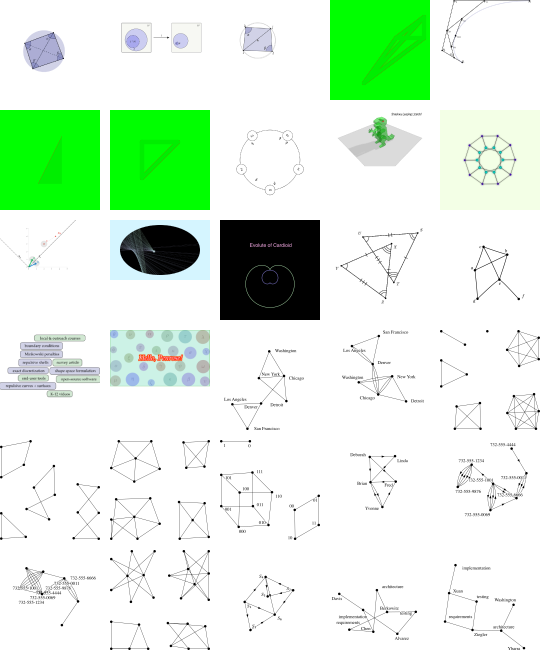
\includegraphics[width=\linewidth]{assets/appendix/Group 9.png}
\pagebreak
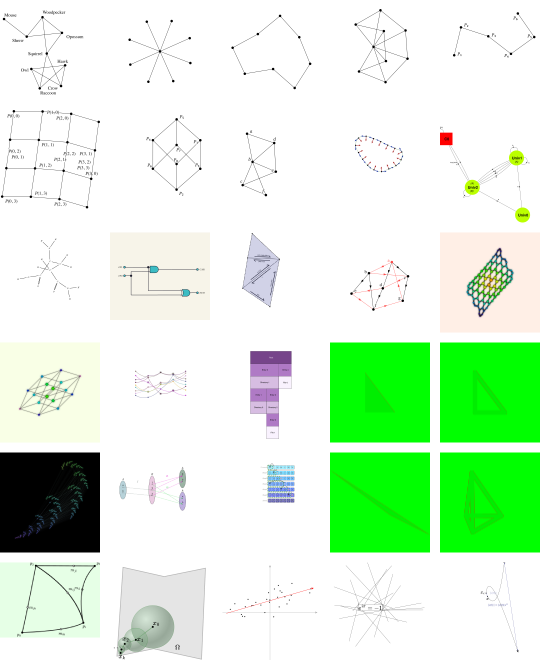
\includegraphics[width=\linewidth]{assets/appendix/Group 10.png}
\pagebreak
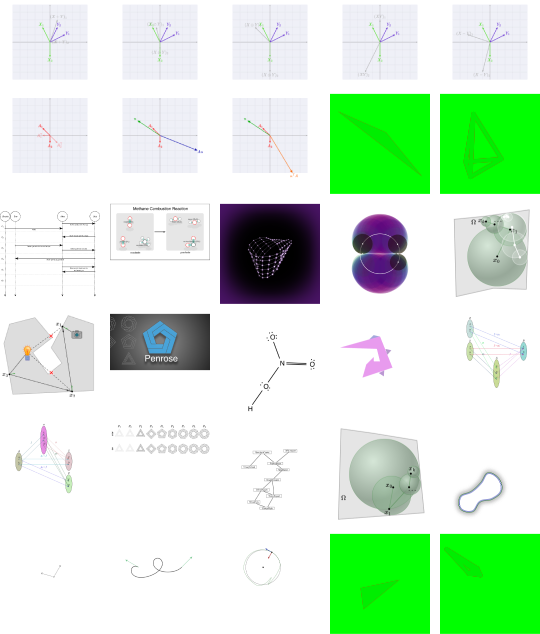
\includegraphics[width=\linewidth]{assets/appendix/Group 11.png}
\pagebreak
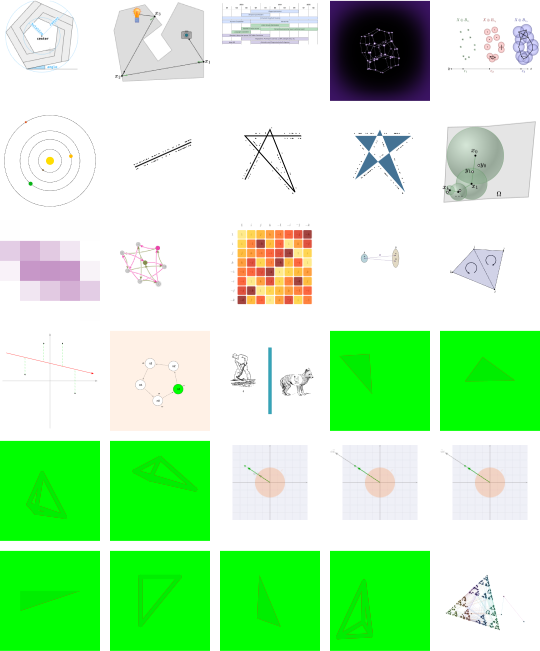
\includegraphics[width=\linewidth]{assets/appendix/Group 12.png}
\pagebreak
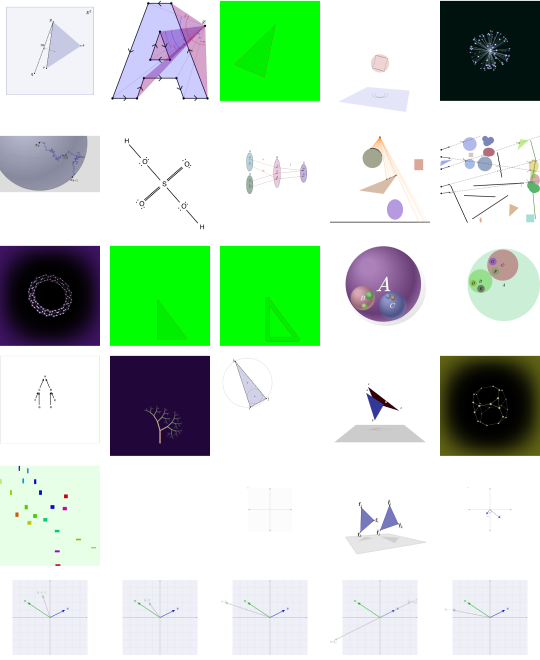
\includegraphics[width=\linewidth]{assets/appendix/Group 13.png}
\pagebreak
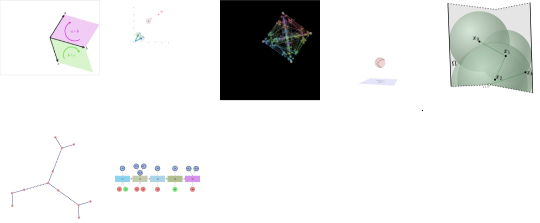
\includegraphics[width=\linewidth]{assets/appendix/Group 14.png}
\pagebreak

